\documentclass[10pt]{article}
\usepackage[margin=0.82in]{geometry}
\usepackage{booktabs,graphicx,amsmath,hyperref,microtype}
\hypersetup{colorlinks=true,urlcolor=blue,linkcolor=blue,pdftitle={CounterScene-3D: Stateful Native-Asset Spatial Evaluation},pdfauthor={Yunfei Lu and GPT-6.1-sol}}
\emergencystretch=2em
\setlength{\parskip}{4pt}\setlength{\parindent}{0pt}
\title{CounterScene-3D: Stateful Native-Asset Spatial Evaluation}
\author{Yunfei Lu \and GPT-6.1-sol}\date{}
\begin{document}\maketitle
\begin{center}\small\href{report_zh.pdf}{Chinese edition}\quad|\quad\href{https://mikelyfei.github.io/CounterScene-3D/}{Interactive benchmark}\end{center}
\begin{abstract}
CounterScene-3D connects executable spatial evaluation with learning-oriented reward diagnosis. Five task families contain thirty native-asset instances and sixty ordered operations. Models respond to consequential changes while preserving actual prior accomplishments. Deterministic geometry, continuous motion checks, auxiliary visual assessment and controlled reward probes distinguish execution readiness, incremental progress and functional completion. A two-model comparison and open-weight selection/refinement studies provide reproducible evidence and concrete directions for curriculum and reward research.
\end{abstract}

\section{Design and contribution}
Spatial reasoning becomes consequential when an action changes what the next decision must preserve. CounterScene-3D retains observations, programs, executed object positions and orientations, feedback and final stage submissions, making this dependency inspectable. Native assets are the actual three-dimensional meshes used for rendering and evaluation.

\textbf{Research foundations.} 3DCodeVerse establishes executable worlds with execution, spatial measurement, visual assessment and repair~\cite{codeverse}. BlenderGym studies code-based reconstruction and generation/verification allocation~\cite{blendergym}; BlenderWorld uses multi-view task-specific visual rubrics~\cite{blenderworld}. SceneScript and VoxPoser provide structured-scene and spatial-action context~\cite{scenescript,voxposer}. Our contribution combines actual state continuity, targeted shortcut audits and separate reward/outcome evidence in a compact protocol. 

Each family has two reproducible scene variants (seeds 0 and 1) and levels L1--L3 requiring one, two and three ordered operations. Instance B-L2-s0 means family B, two operations, seed 0. A retains dataset labels k06/k14/k34 for L1/L2/L3 respectively; these labels do not count operations. Later operations introduce observations and preservation obligations.

\textbf{A: relocation and restoration.} Move a work surface, park its payloads at the original floor location, restore measured surface-relative offsets, then update another work area while preserving the restoration. Explicit targets distinguish goal completion from generic collision clearance.

\textbf{B: progressive repair.} Repair witnessed interpenetrations as work zones become editable. Earlier repairs and unreleased zones remain fixed. Declared future faults are temporarily permitted; the final operation enforces all mandatory constraints and jointly feasible preferences. Models must identify preferences that cannot be satisfied.

\textbf{C: changing-view reconstruction.} Reconstruct native instances from calibrated views, then update after substantial target changes and new oblique observations. Additional views are budgeted. Hidden-view agreement, every-object centre accuracy and native physical rules jointly determine success.

\textbf{D: stateful manipulation.} Grasp distinct balls, deliver and release them, then reach onward waypoints. Later operations inherit actual final joint angles and released-object positions; earlier releases become obstacles. Measured offsets connect command angles to physical motion.

\textbf{E: misleading diagnostics.} Repair actual faults while public feedback contains witnessed wrong verdicts, omissions, noise or hidden pairs. Geometry measurements support verification. Repair outcomes and diagnosis are reported separately, enabling controlled feedback studies.

\begin{figure}[htbp]\centering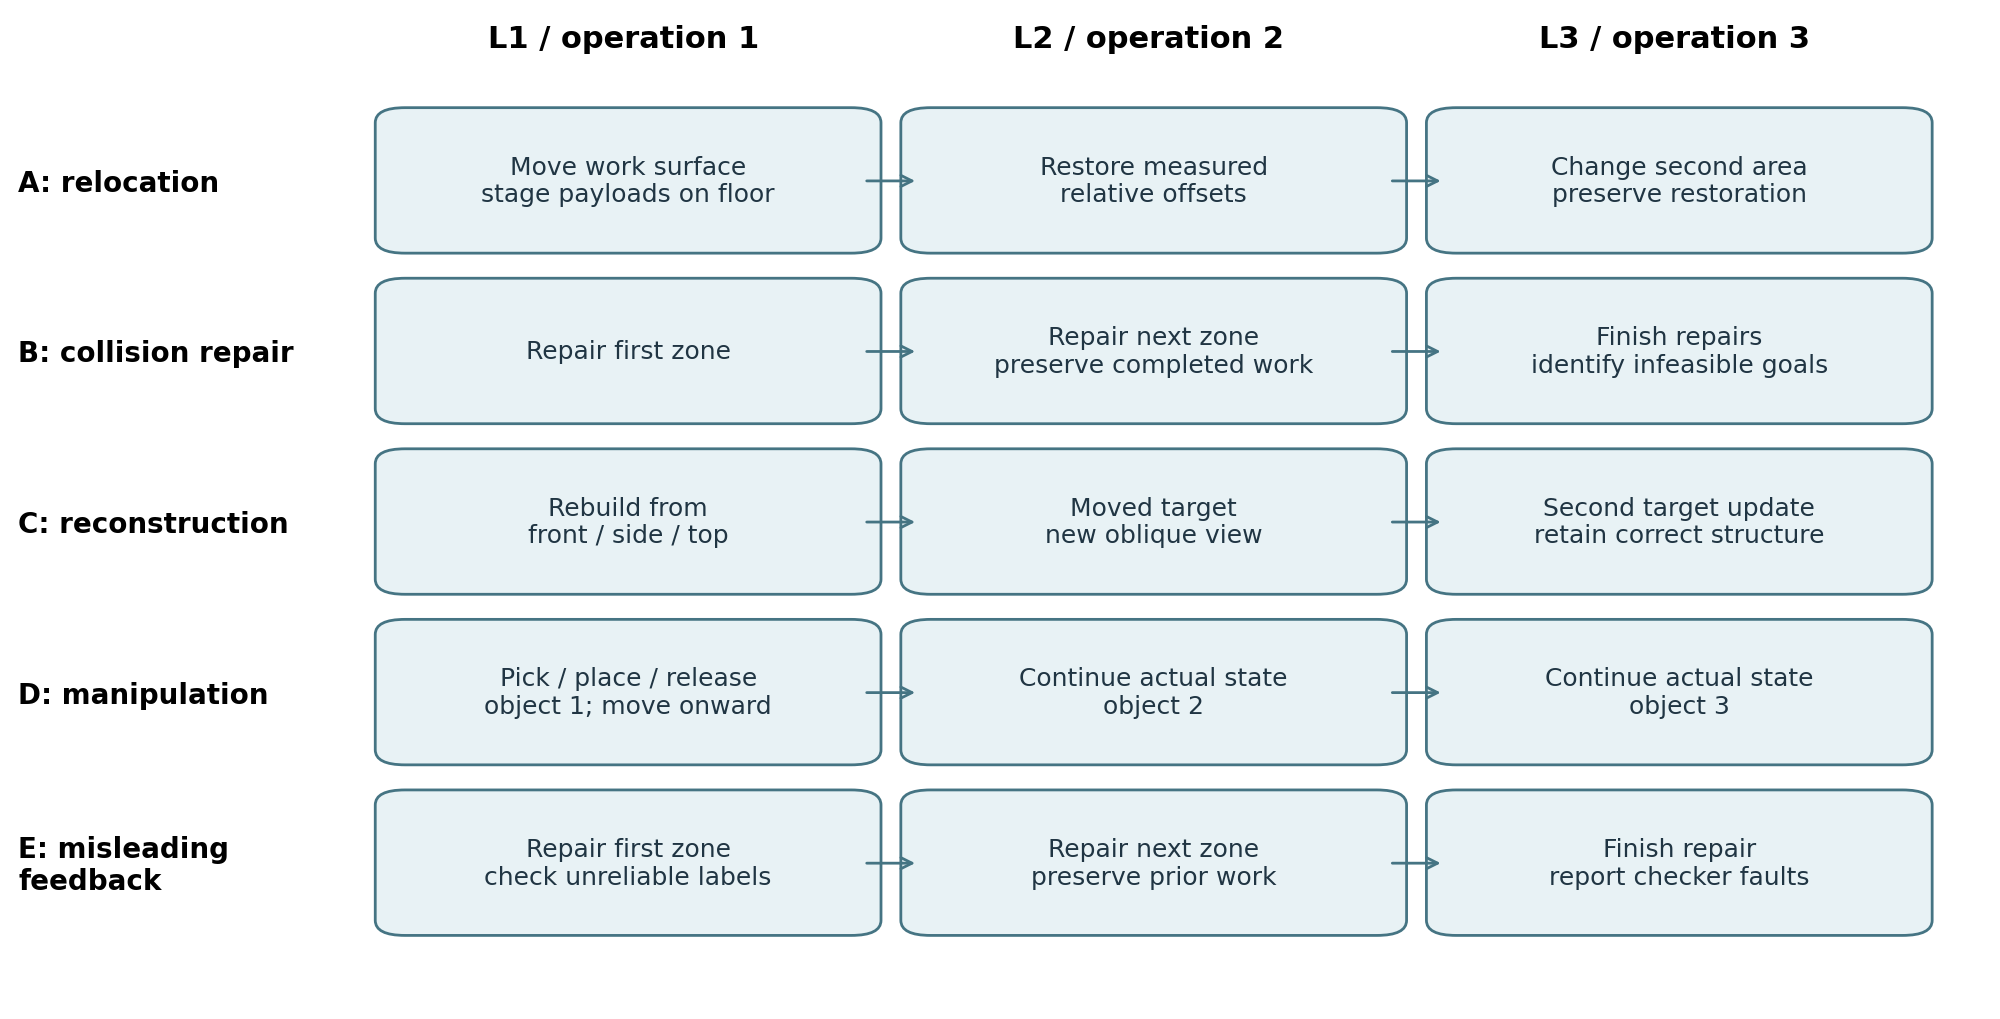
\includegraphics[width=\linewidth]{figures/benchmark_design.png}\caption{Implemented dependencies across five families. Subsequent operations preserve prior accomplishments.}\end{figure}

\section{Execution and measurement}
Participants emit restricted Python returning complete native placements or controller payloads. Bounded arithmetic and collections are allowed; imports, attributes, files and network access are denied. Fixed catalogue identity and proportions bind programs to actual assets.

Gold denotes evaluator-verified reference solutions. Replaying these solutions from version-bound stage files verifies feasibility using actual meshes. Shortcut controls challenge stale answers, fixture-only patches, omitted observations and earlier-program reuse. 

Static checks use actual meshes for support, boundaries, contact and intersection. Relocation and reconstruction path checks use conservative bounding volumes around mesh components. D additionally checks continuous arm, tool and payload clearance, limits, grasp/release events and resting objects. A path passes only when these checks establish clearance. The evaluated scope is geometric and kinematic; richer dynamics are an extension opportunity.

Strict success requires every operation and preservation obligation; later corrections retain earlier outcomes in episode scoring. C requires silhouette intersection-over-union (IoU: overlap area divided by union area), averaged over objects and evaluator-only cameras, of at least 0.8, plus every mesh bounding-box centre within 0.05 metres of its target. D requires the complete continuous/event contract. Infrastructure interruptions are excluded; journaled responses and exact program bytes support repeatable recovery.

\begin{figure}[htbp]\centering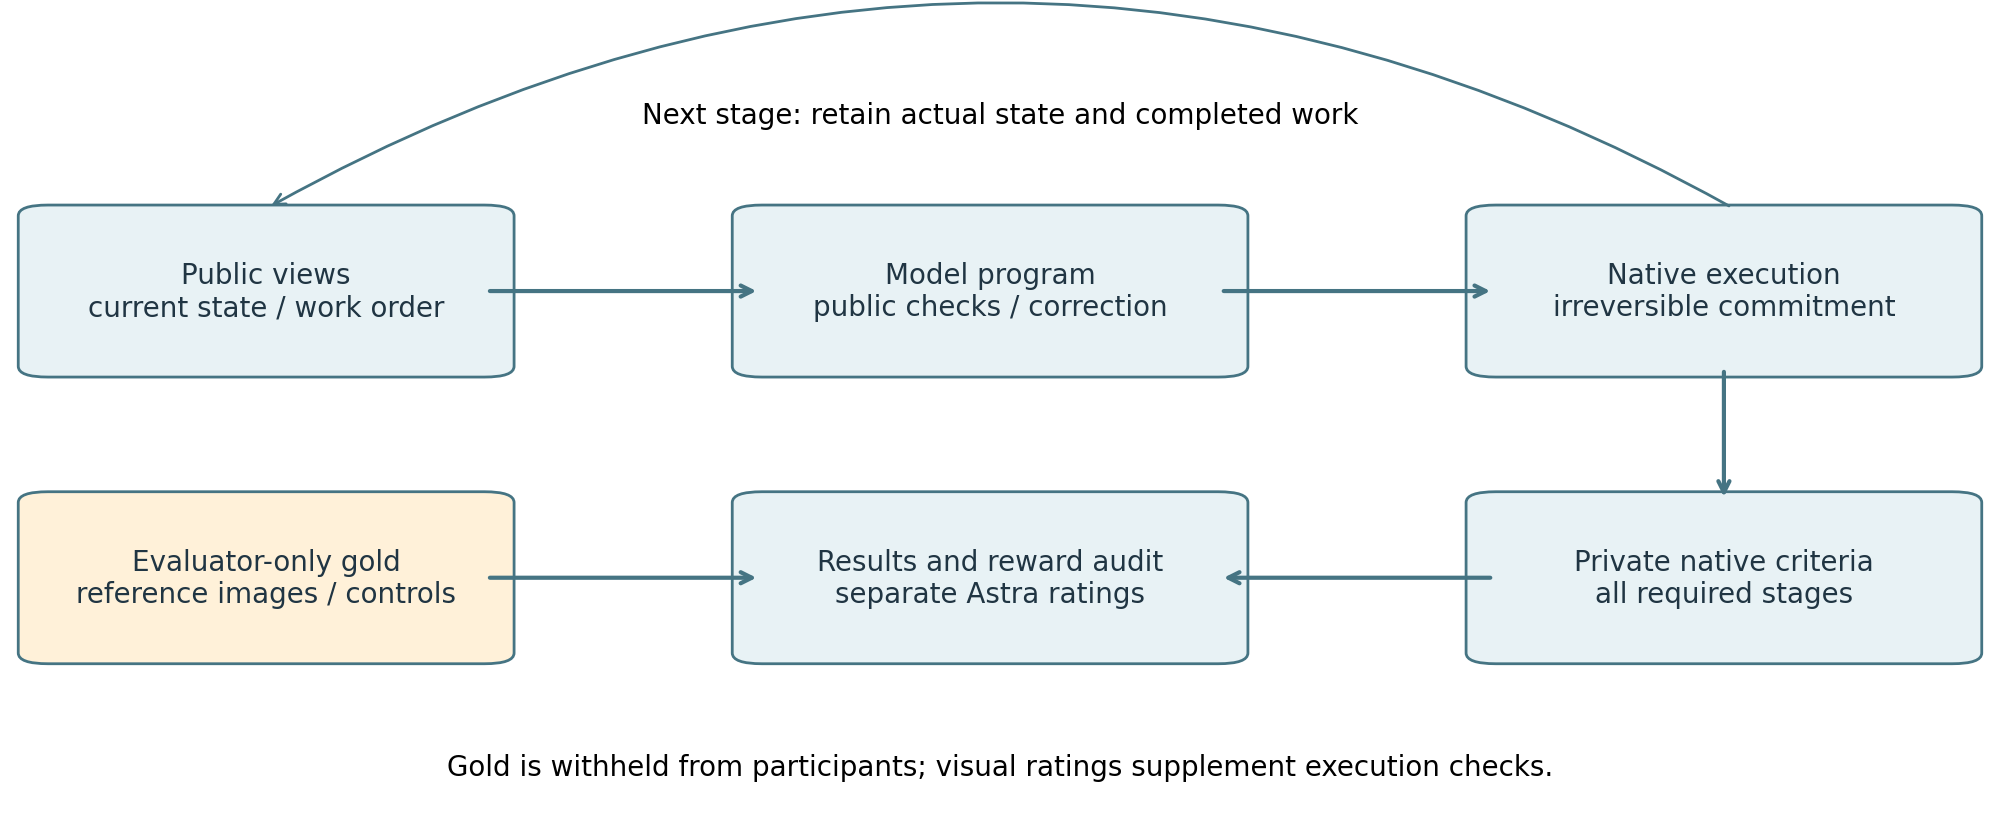
\includegraphics[width=\linewidth]{figures/evaluation_flow.png}\caption{Public observations guide decisions; evaluator-only targets support separate outcome checks.}\end{figure}

\section{Comparison protocol and results}
GPT-6.1 Sol and Claude Opus 5.5 use medium reasoning, up to 8,000 output tokens and fourteen actions per operation. A trajectory comprises all operations for one instance. Thirty instances per model yield sixty primary trajectories; ten additional L3 requests form an independent-generation panel. Primary means describe six instances per task/model. Generation variance, fixed-output rescoring and visual-judge repetition remain distinct. The extension adds five completed exploratory controls; one interrupted continuation is excluded.

\section{Results and observable failure modes}

All 70 planned model trajectories completed without infrastructure interruption. The table reports six primary instances per task/model: Strict is the episode success rate; Shaped is mean evaluator reward (0--1), including safe partial progress. Results describe this development cohort.

\begin{center}\small

\begin{tabular}{llrrr}\toprule

Task & Model & $n$ & Strict & Shaped \\ \midrule

A & Claude & 6 & 1.000 & 1.000 \\

A & GPT & 6 & 1.000 & 1.000 \\

B & Claude & 6 & 0.833 & 0.982 \\

B & GPT & 6 & 0.833 & 0.981 \\

C & Claude & 6 & 0.333 & 0.432 \\

C & GPT & 6 & 0.500 & 0.580 \\

D & Claude & 6 & 1.000 & 1.000 \\

D & GPT & 6 & 1.000 & 1.000 \\

E & Claude & 6 & 0.833 & 0.765 \\

E & GPT & 6 & 1.000 & 0.912 \\

\bottomrule\end{tabular}\end{center}

Across 10 completed independent-request panels, shaped-reward population variance ranges from 0.0000 to 0.2223. This is generation variability, not repeat-scoring variance; more independent generations would improve uncertainty estimates.

\begin{center}\small

\begin{tabular}{lrr}\toprule

Observed failure category & GPT & Claude \\ \midrule

checker diagnosis & 6 & 6 \\

hard constraint violation & 1 & 1 \\

hidden view grounding & 0 & 4 \\

metric grounding & 2 & 4 \\

native physical conflict & 3 & 3 \\

native relation violation & 0 & 1 \\

tool or program error & 11 & 1 \\

\bottomrule\end{tabular}\end{center}

Counts are primary trajectories with observed issues; labels overlap. Diagnostic errors include geometrically successful episodes; tool errors are invalid actions.

In B-L2-s0, both models resubmit unchanged programs after reported mandatory-constraint failures: the earlier stage succeeds, but final repair fails. This behavior motivates feedback-use studies.

In C-L2-s0, Claude passes initial reconstruction but misses hidden-view and position thresholds after the target changes, using thirteen actions without querying another view.

In C-L2-s1, GPT passes silhouette and centre checks but retains a physical conflict at stage one. Stage two passes; episode scoring preserves the earlier error, demonstrating the value of cumulative, multidimensional acceptance. Claude shares the physical conflict and additionally misses position thresholds.

E-L3-s1 separates repair from diagnosis: GPT meets 26/26 native relations and detects 2/4 checker faults; Claude meets 25/26 and detects 0/4. Separate metrics make both capabilities inspectable.

\paragraph{Reward evidence.}

Calibration across 30 instances and 360 repeated scores establishes repeatability: maximum fixed-control shaped-reward variance is 0.0000, and ordering checks all pass. Scorer repeatability and generation variance are measured separately.

The completed Qwen study comprises 10/10 pools with four candidates each. Public-reward selection raises mean independently audited hidden quality from 0.000 for the first candidate to 0.200. Observed gains occur in A. Exact replay preserves selection and ties.

E makes feedback alignment directly auditable: selected public reward averages 0.300, while hidden quality is 0.000. This identifies feedback-validation and curriculum targets.

GPT-6 Astra, the auxiliary vision-language judge, quantifies visual-assessment consistency: fixed-image sample variances range from 0.0000 to 0.0093 across 15 control artifacts, with mean coverage (fraction of rubric items scored) 0.906. Native checks identify 7 functional failures with visual scores of at least 0.75, supporting complementary visual and executable evaluation.

Weak visual-control ordering holds in 5/5 observed families. Gold strictly exceeds stale in 5/5 families. Weak ordering allows ties: reference scores exceed or equal safe partial scores, then stale scores. This validity diagnostic guides rubric refinement.

Controlled selection and acceptance support learning-oriented reward research.

\begin{figure}[htbp]\centering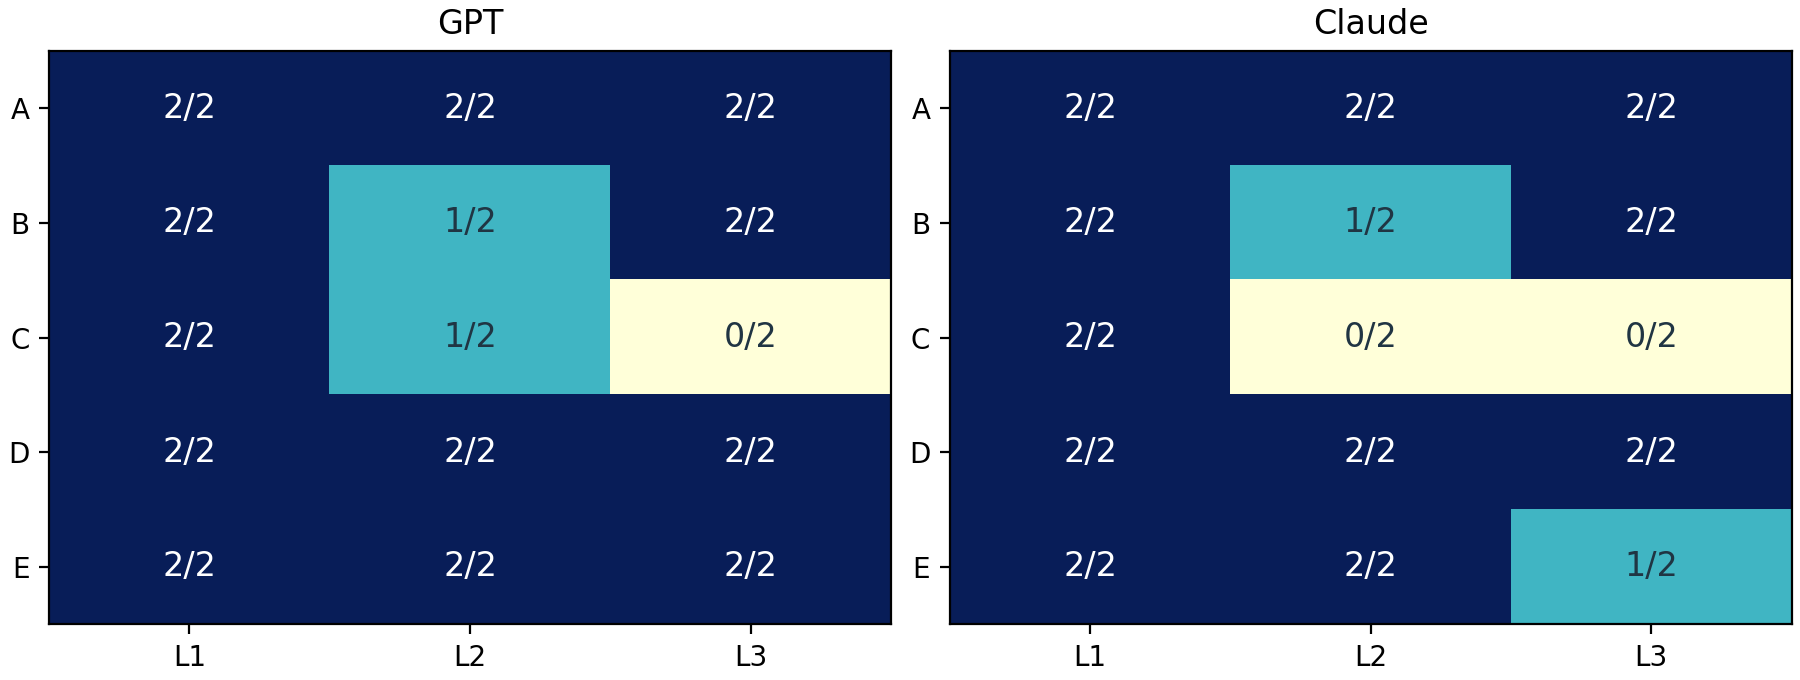
\includegraphics[width=.88\linewidth]{figures/performance_by_level.png}\caption{Primary strict successes by level, with two seeds per cell, characterize the current development cohort.}\end{figure}
\begin{figure}[htbp]\centering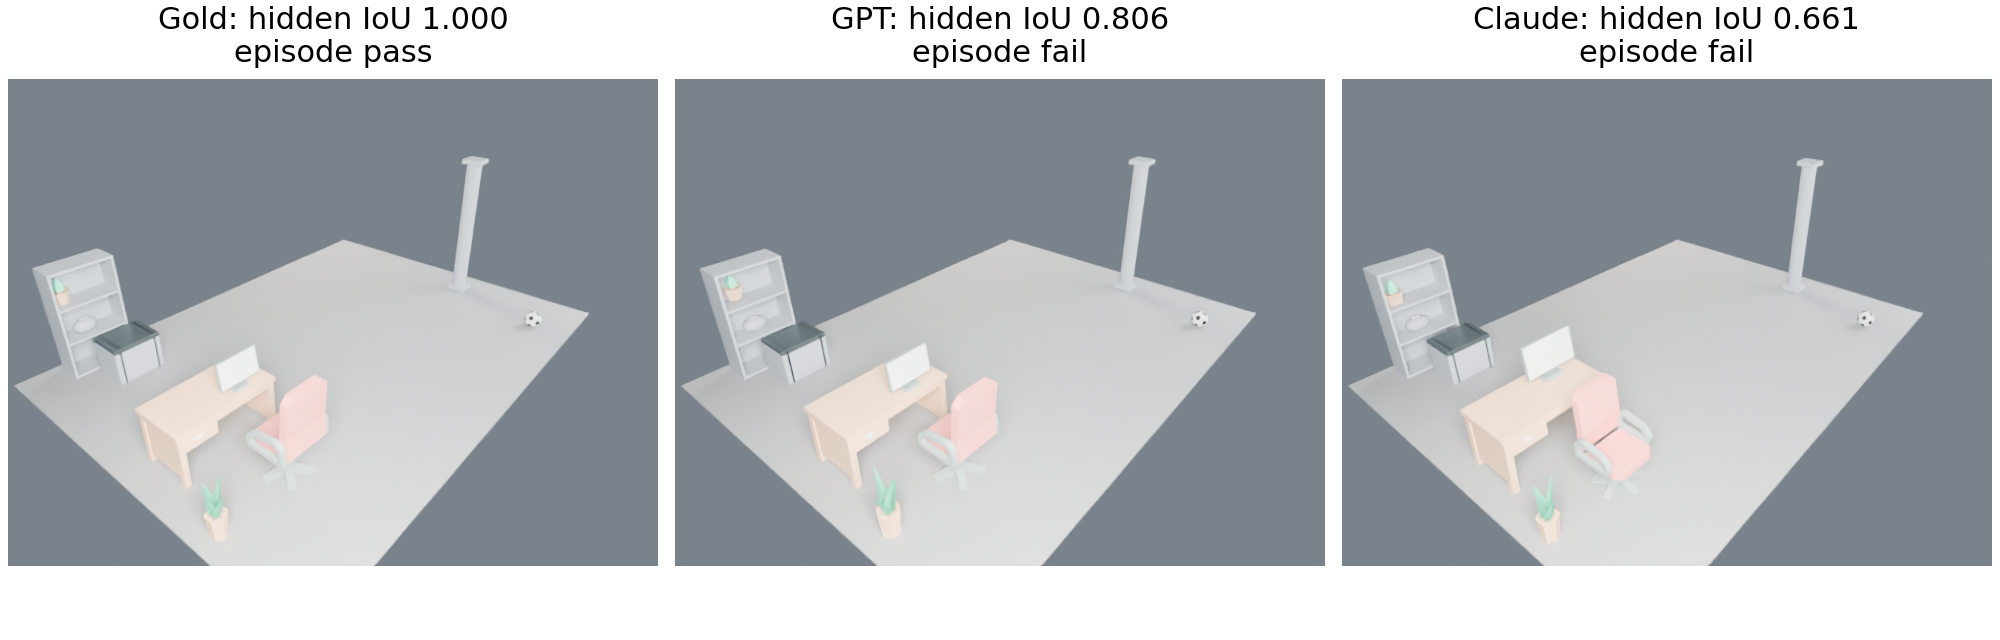
\includegraphics[width=\linewidth]{figures/reconstruction_comparison.png}\caption{C-L3-s0 reference and executed renders. Hidden IoU complements metric and native physical criteria.}\end{figure}

\section{Reward diagnosis and learning implications}
Rubrics as Rewards and AdvancedIF/RIFL motivate explicit criteria and aggregation~\cite{rar,rifl}. VideoEdit studies when finer credit assignment supports outcomes~\cite{videoedit}; we therefore inspect behavioral progress without rewarding additional calls.

Per-stage deterministic reward $R_{\rm det}$ is 1 for functional success under mandatory safety and preservation checks, and 0 otherwise. $R_{\rm shaped}$ equally averages applicable function, constraint, preservation, diagnosis, operation, reconstruction and motion components. Episode rewards average required stages; missing stages contribute zero, and inapplicable dimensions are omitted. These mandatory checks gate reward while permitting safe partial progress.

Reference solutions, empty outputs, reused earlier answers (or stationary motion), and safe partial solutions test expected score ordering. A five-output native-repeat subset independently re-executes one GPT output per family: complete stage measurements match across two executions each.

Astra anonymously compares reference and candidate images for identity/layout, visible support, clearance and goal match. Uncertain items remain missing; coverage is the fraction of rubric items assigned a score. D uses representative trajectory frames. Repeated images characterize judge variability; broader judge/human checks address known model-judge biases~\cite{judge}. Visual evidence complements functional acceptance.

The original Qwen3.5:9B study uses a nine-billion-parameter open-weight model with Q4\_K\_M quantization. Each of ten pools contains four generated candidates; the highest public-tool reward selects one, with ties resolved by generation order. Hidden quality is its independently evaluated shaped reward, withheld from selection. The extension introduces matched proposal/refinement arms and separately exposes the actual scalar evaluator reward.
\paragraph{Extended learning diagnostics.}
Public-reward selection yields mean hidden quality 0.20 versus 0.075 under uniform random selection, with gains concentrated in A. Five feedback/view controls compare execution status only, detailed constraint reports, or a scalar score; fixed views provide initial images only, while active access allows additional queries. GPT solves B-L2-s0 with execution-only feedback; fixed-view C-L2-s0 succeeds in 10 calls versus 26 with active access. These exploratory cases guide larger matched panels; one incomplete Claude C continuation is excluded.

Eight matched-budget arms compare independent proposals with public-feedback refinement across C, D, two-operation A and E, using three proposals per stage. A formatting adapter uses only public information, without target answers. Native scoring accepts 26 of 30 proposals, allowing the benchmark to isolate geometric planning from interface competence. With strict completion at 0/8 and zero admissible reward for 29 proposals, the cohort identifies curriculum and denser-feedback targets under unchanged acceptance criteria.

Two D studies expose shaped reward, each adding two generations to either the matched first proposal or the model's first publicly executable proposal. Both retain starting reward and remain below strict completion. A separate safe D candidate earns 0.4 with transfer incomplete, separating partial progress from success. Training and held-out evaluation can test these reinforcement learning (RL) directions.

\paragraph{Per-dimension robustness.}
The table makes each attack and guard explicit. Bounded means susceptible to shortcuts within the stated checks and tolerances; classifications apply to this tested domain. Full examples and mitigations accompany the task packages and study data.
\begin{center}\small\begin{tabular}{p{.20\linewidth}p{.17\linewidth}p{.52\linewidth}}\toprule
Dimension & Class & Attack; verification guard \\ \midrule
Program/identity & Hard-to-hack & Malformed or substituted assets; interpreter and identity checks. \\
Physics/contact & Bounded & Contact tolerances; actual mesh and fail-closed unknowns. \\
Operation goals & Bounded & Clear scene but missed operation; explicit targets. \\
Soft/diagnosis & Bounded & Invented impossibility; joint feasibility checks and claim checks. \\
Metric grounding & Bounded & Matching silhouettes, wrong centres; conjunctive metric audit. \\
Trajectory/events & Bounded & Endpoint shortcuts; continuous checks and actual releases. \\
Edit/preservation & Bounded & Unchanged low-edit answer; active goals and preservation. \\
Checker agreement & Bounded & False passes; separate geometry and diagnosis. \\
Visual quality & Qualitative & Occlusion or appearance; auxiliary role and coverage. \\
Target access & Bounded & Hidden-file access; restricted public interface. \\ \bottomrule
\end{tabular}\end{center}

\begin{figure}[htbp]\centering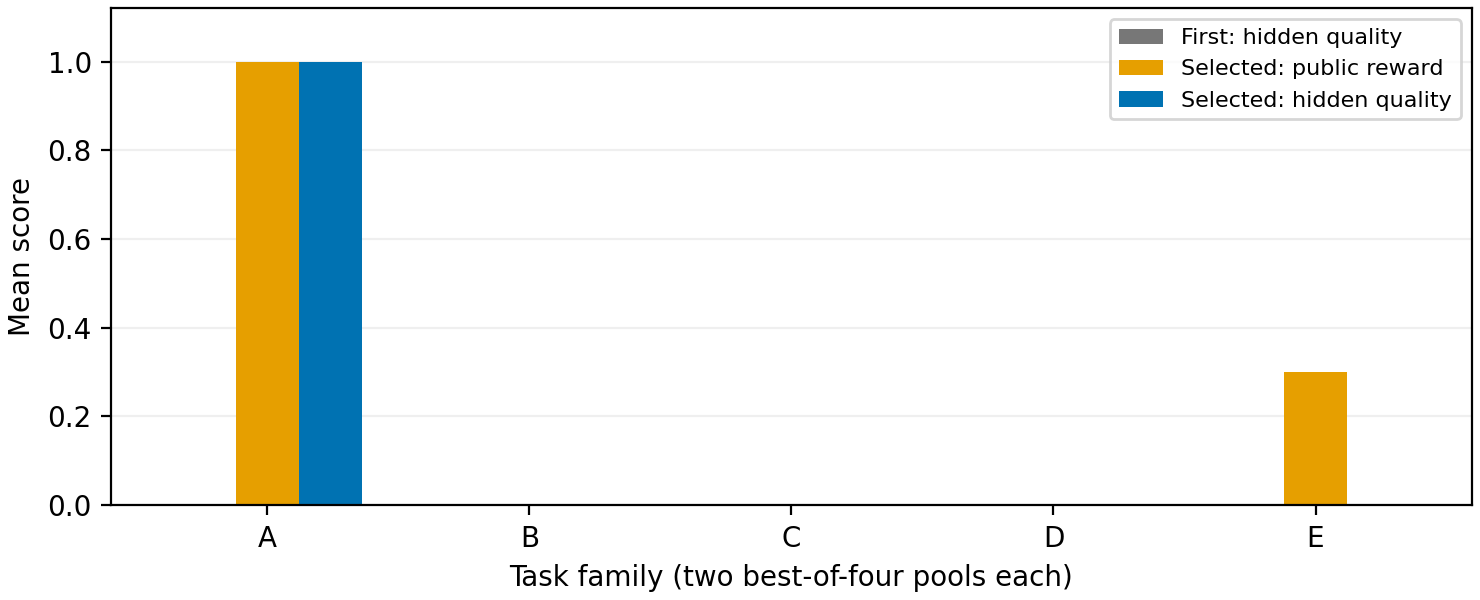
\includegraphics[width=.85\linewidth]{figures/qwen_reward_quality.png}\caption{Original best-of-four selection and withheld quality. A supplies the observed gain; expanded diagnostics identify subsequent curriculum targets.}\end{figure}

\section{Reproducibility and areas for improvement}
Self-contained packages retain public inputs, evaluator targets, gold, scorers, native assets and licenses. One command reconstructs rewards, tables, statistics and supplementary selection; optional native replay executes retained programs. Published development logs are redacted to remove private information.

\textbf{Scale and coverage.} Expand reserved scenes, catalogues, seeds and matched feedback/view conditions. The present extension is exploratory and includes one administrative exclusion. Larger panels and matched interface/context settings will support stronger causal and generalization estimates.

\textbf{Learning studies.} The safety gate yields sparse feedback for this initial policy. Develop curricula from executable placements to coupled geometry and longer horizons, compare progress-sensitive feedback under fixed acceptance criteria, and run longer adaptive optimization followed by short RL studies. 

\textbf{Physical and visual scope.} Calibrate conservative enclosure rejections with independent mesh tests, then add friction, forces and grasp dynamics. Extend blinded judge/human review and event-sensitive clips. Match the smaller-model scaffold to full motion and physical-pair diagnosis interfaces before broader comparisons.

\textbf{Reward design.} Compare weights and attack policies on reserved outcomes. Track reward gaps before and after optimization to distinguish feedback bias from learned exploitation. Per-dimension evidence supports reproducible tests of functional quality under optimization.



\clearpage\section{Motion evidence}
These trajectories expose calibration, pickup, release and onward movement as separate obligations. Earlier releases remain obstacles. Joint-derived paths and representative native frames make the relationship between plausible endpoints and certified transfers inspectable.
\begin{figure}[ht!]\centering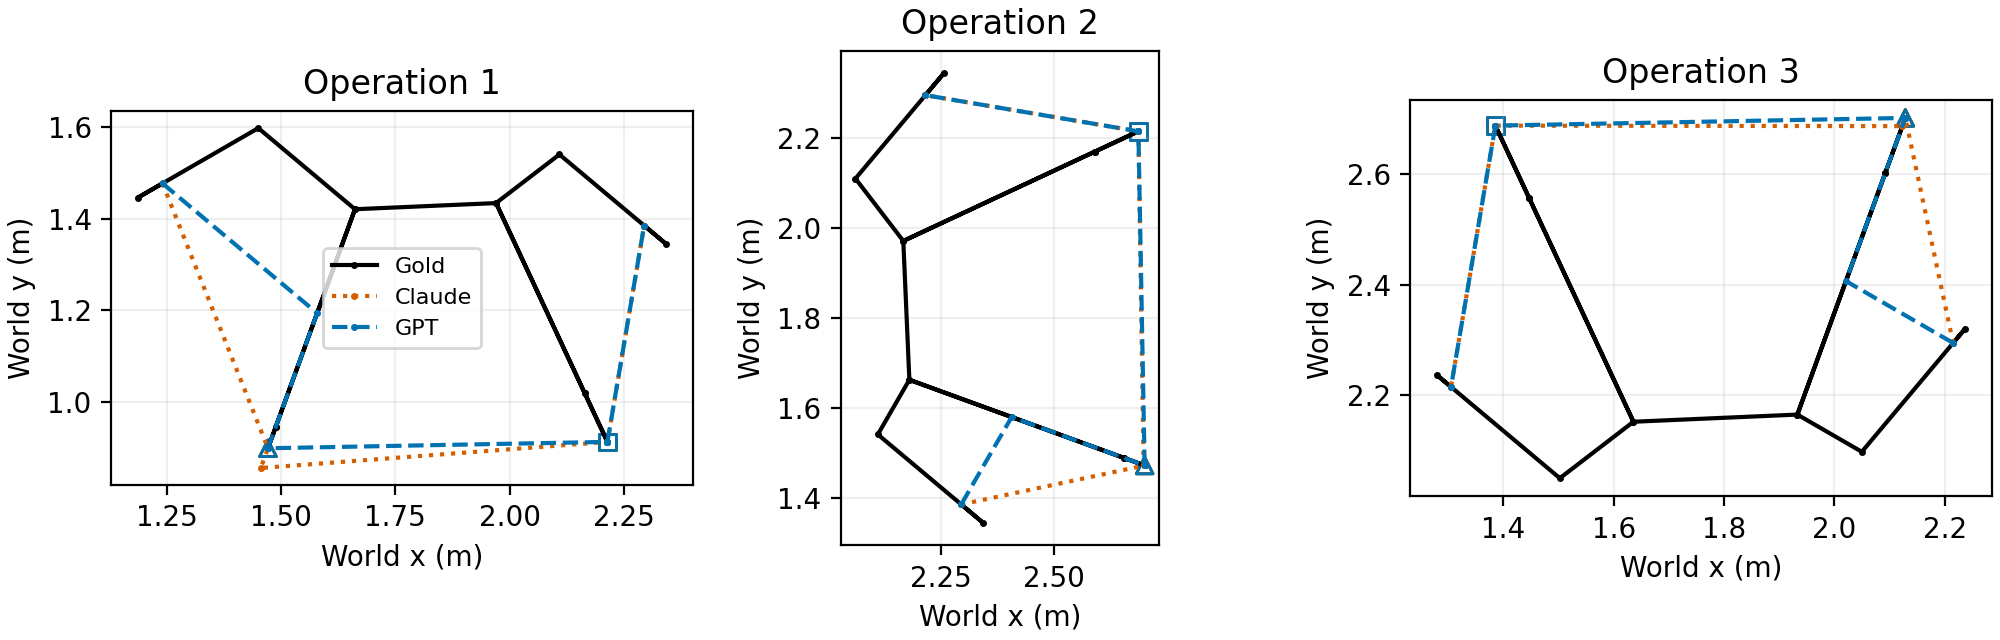
\includegraphics[width=\linewidth]{figures/motion_comparison.png}\par\bigskip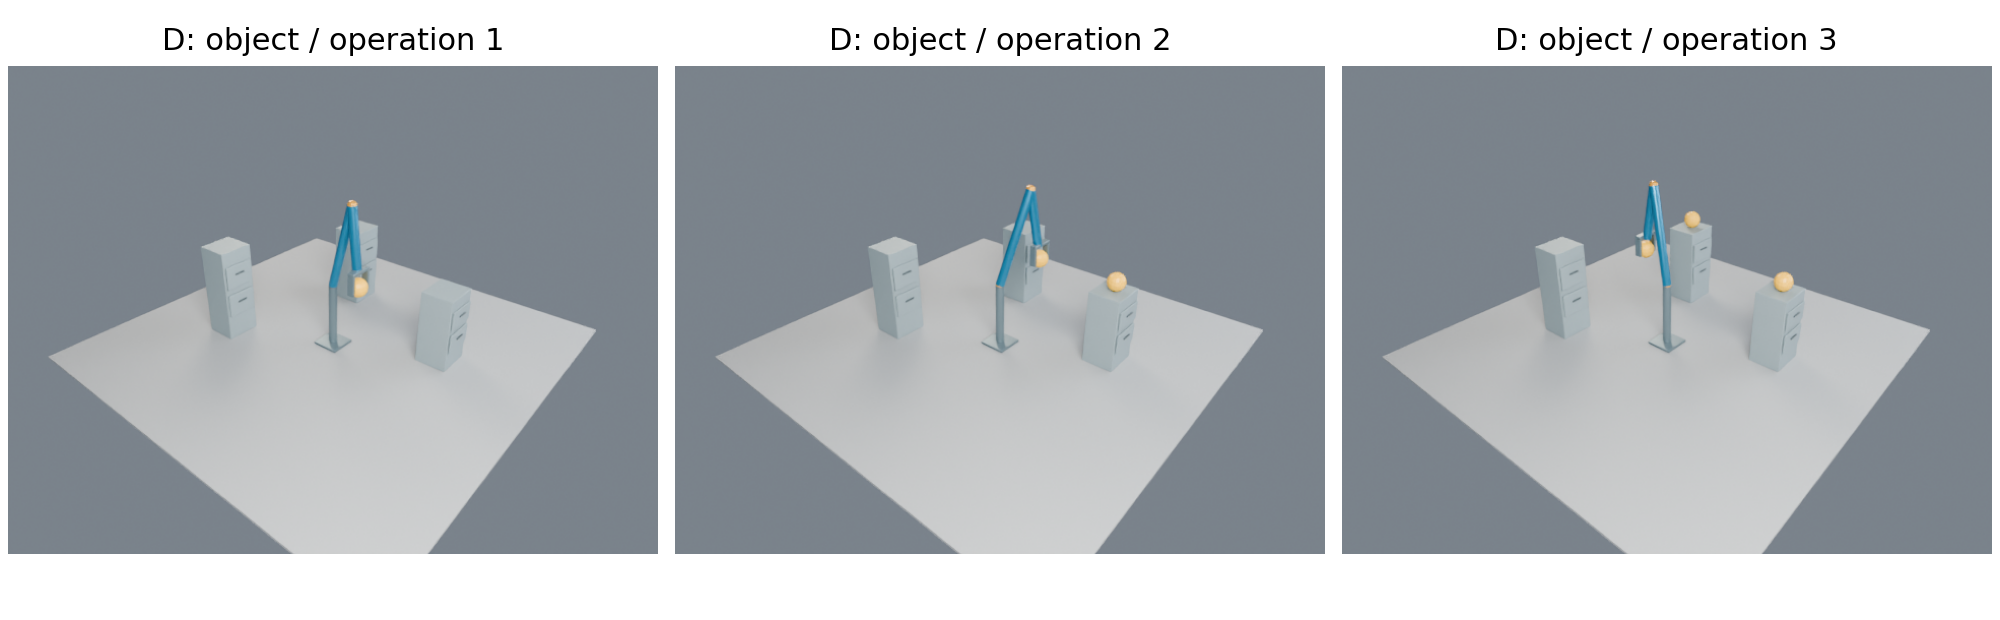
\includegraphics[width=\linewidth]{figures/motion_native_examples.png}\caption{D-L3-s0 joint-derived trajectories and representative native transfer frames. Triangles mark grasps, squares releases; continuous collision and event checks establish motion validity.}\end{figure}
\clearpage\section{Benchmark examples}
\begin{figure}[ht!]\centering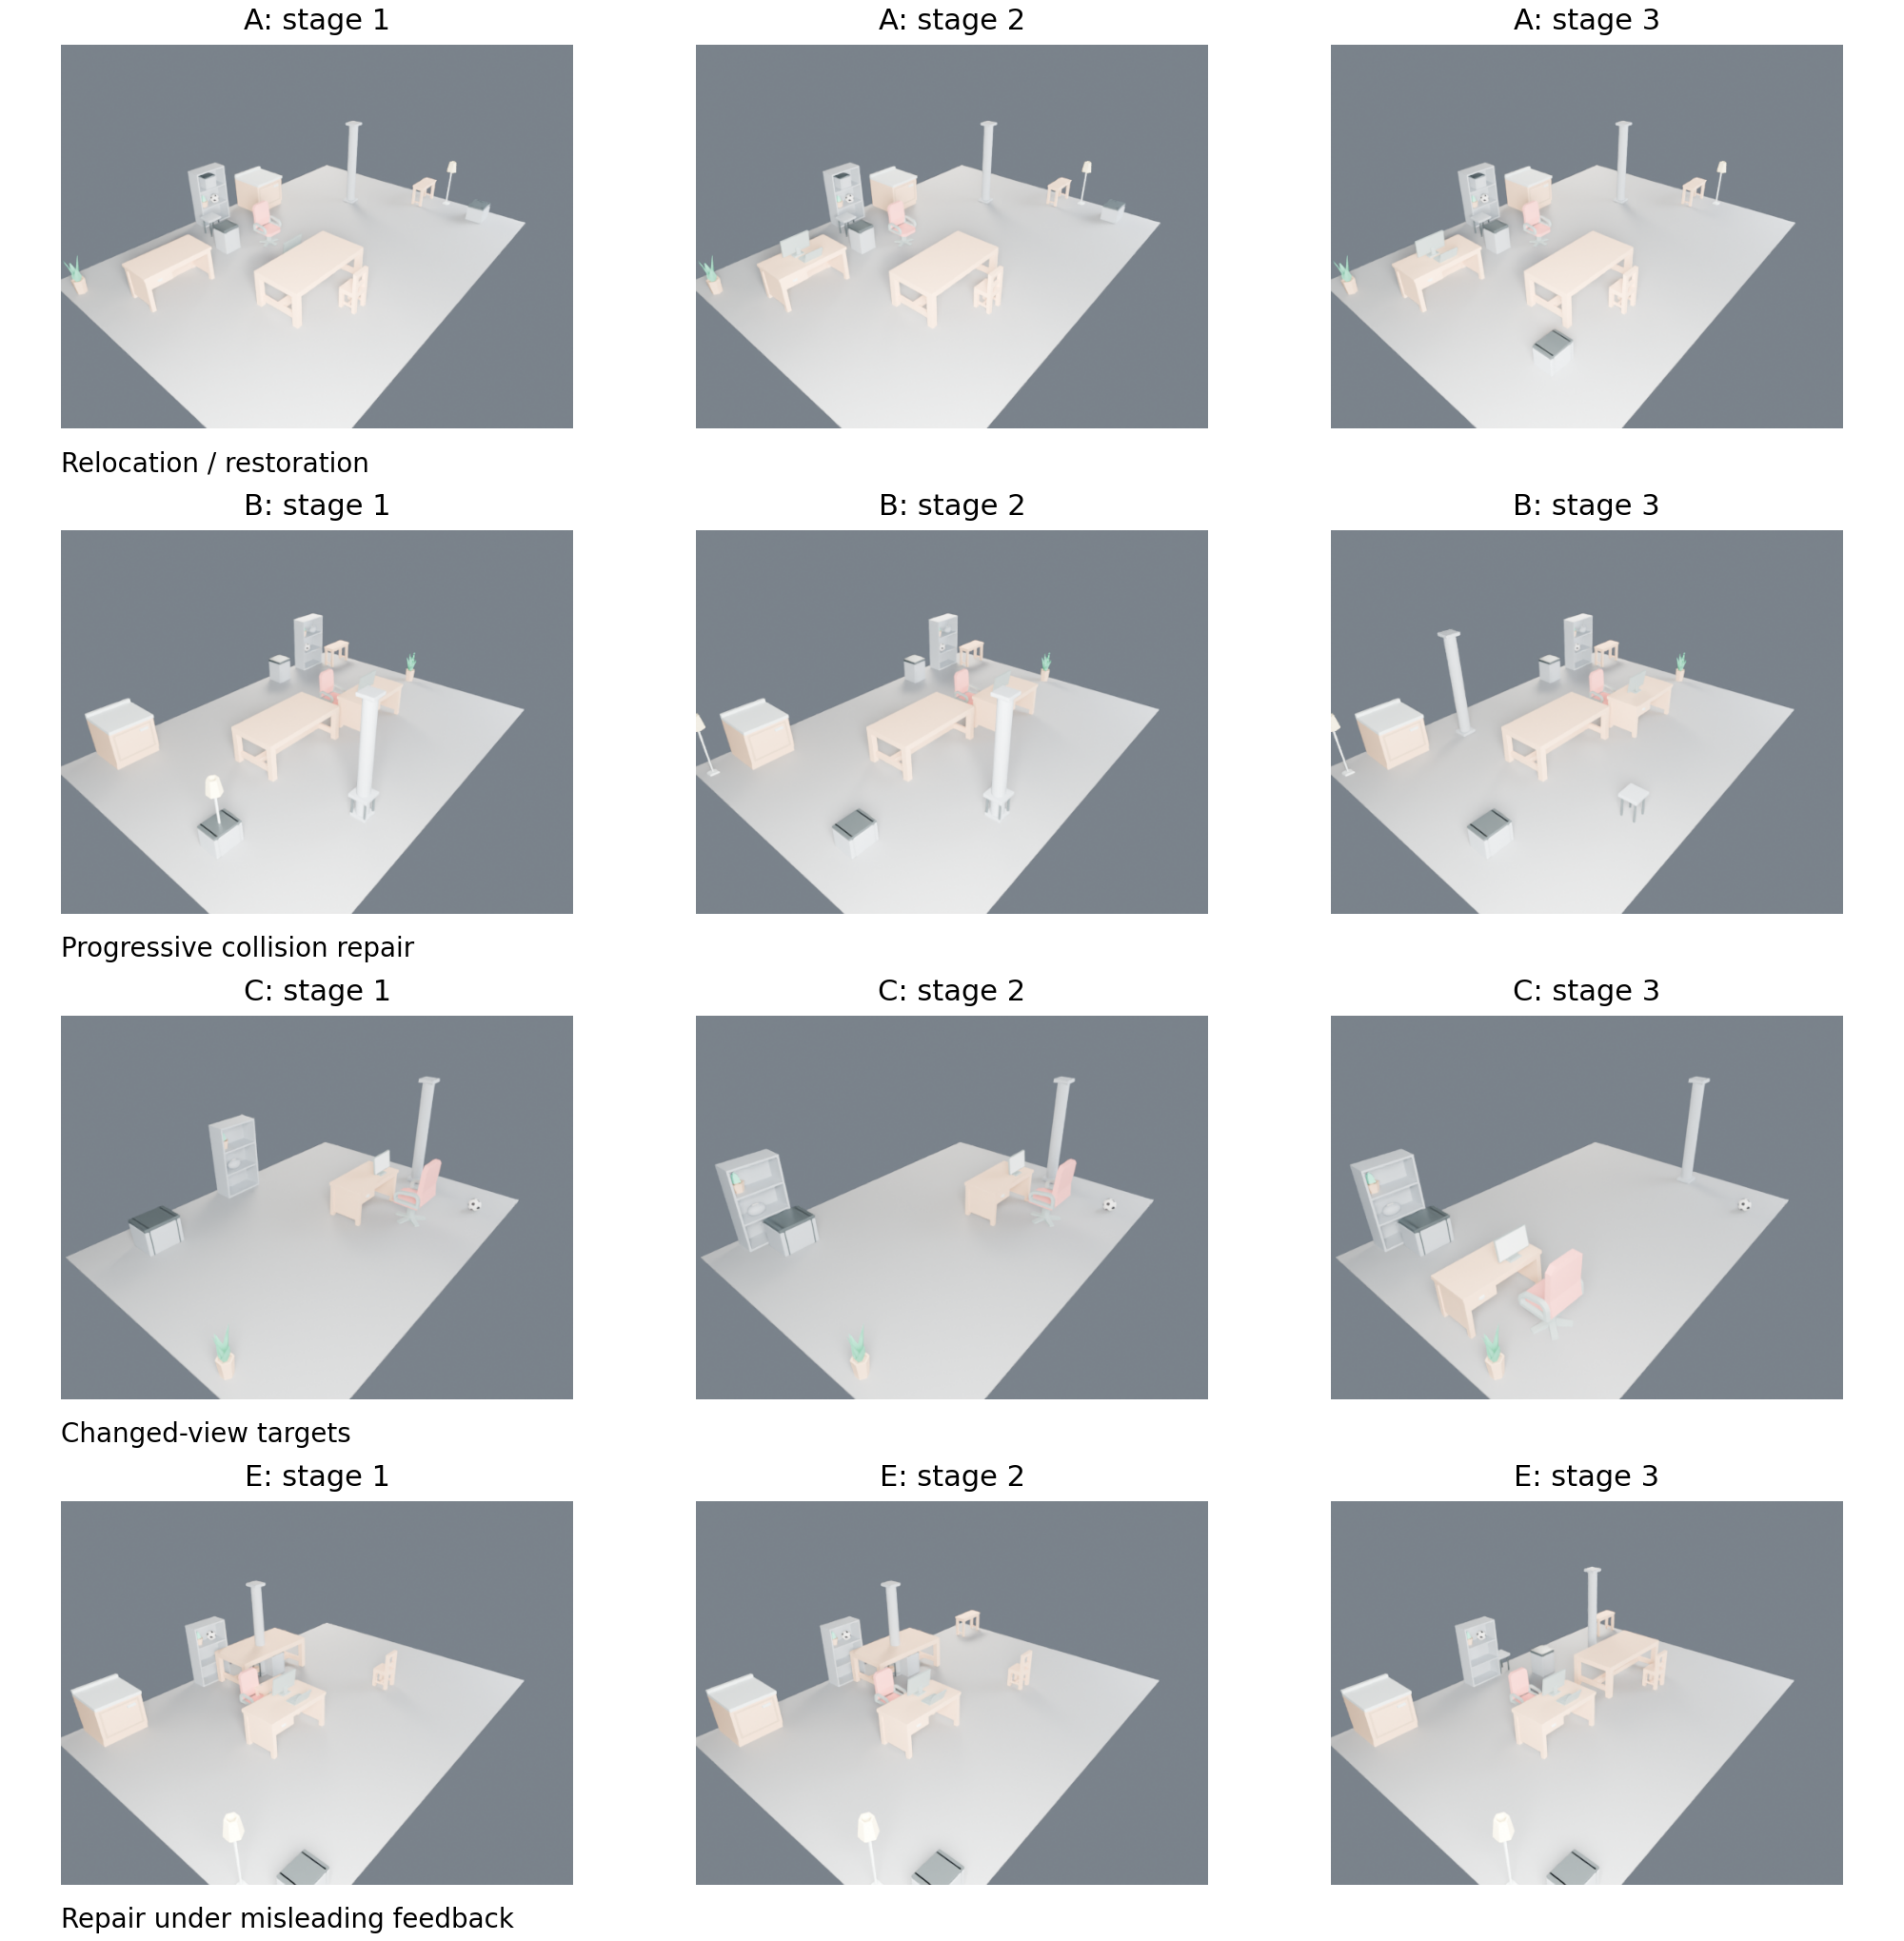
\includegraphics[width=.98\linewidth,height=.64\textheight,keepaspectratio]{figures/benchmark_examples.png}\caption{Actual three-stage gold witnesses for A/B/C/E. B/E intermediate states retain explicitly declared future faults.}\end{figure}
\clearpage\begingroup\small
\begin{thebibliography}{99}
\bibitem{codeverse} Gao et al. 3DCodeVerse: Exploring 3D Worlds as Code. 2026 preprint. \url{https://arxiv.org/abs/2610.22341}. Official harness: \url{https://github.com/gaoypeng/3dcodeverse/tree/main/harness}.
\bibitem{blendergym} Gu et al. BlenderGym: Benchmarking Foundational Model Systems for Graphics Editing. CVPR, 2025. \url{https://arxiv.org/abs/2504.01786}.
\bibitem{blenderworld} Fang et al. BlenderWorld: Benchmarking Visual Agents for 3D Creation from Real-World References. 2026 preprint. \url{https://arxiv.org/abs/2610.23986}.
\bibitem{scenescript} Avetisyan et al. SceneScript: Reconstructing Scenes With An Autoregressive Structured Language Model. 2024. \url{https://arxiv.org/abs/2403.13064}.
\bibitem{voxposer} Huang et al. VoxPoser: Composable 3D Value Maps for Robotic Manipulation with Language Models. 2023. \url{https://arxiv.org/abs/2307.05973}.
\bibitem{rar} Gunjal et al. Rubrics as Rewards: Reinforcement Learning Beyond Verifiable Domains. 2025 preprint. \url{https://arxiv.org/abs/2507.17746}.
\bibitem{rifl} He et al. AdvancedIF: Rubric-Based Benchmarking and Reinforcement Learning for Advancing LLM Instruction Following. 2025 preprint. \url{https://arxiv.org/abs/2511.10507}.
\bibitem{videoedit} Zhao et al. When Fine-Grained Credit Assignment Helps and Hurts: Multimodal Agentic Reinforcement Learning through Video Editing. 2026 preprint. \url{https://arxiv.org/abs/2610.35497}.
\bibitem{judge} Zheng et al. Judging LLM-as-a-Judge with MT-Bench and Chatbot Arena. NeurIPS Datasets and Benchmarks, 2023. \url{https://arxiv.org/abs/2306.05685}.
\end{thebibliography}\endgroup\end{document}
